%root = ../
\documentclass[a4paper,11pt]{report}
\usepackage{float}
\usepackage[italian]{babel}
\usepackage[T1]{fontenc}
\usepackage[utf8]{inputenc}
\usepackage{geometry}
\usepackage{graphicx}
\usepackage{hyperref}
\usepackage{enumitem}
\usepackage{xcolor}
\usepackage{listings}
\usepackage{tikz}
\usepackage{lmodern}
\usepackage{amsmath,amssymb,amsfonts,amsthm}
\usepackage{booktabs}
\usepackage{tikz-uml}
% Definizione colori stile IDE / Documentazione
\definecolor{codebg}{RGB}{248, 250, 252}
\definecolor{codeframe}{RGB}{226, 232, 240}
\definecolor{primary}{RGB}{30, 41, 59}
\definecolor{keywordcolor}{RGB}{37, 99, 235}
\definecolor{stringcolor}{RGB}{13, 148, 136}
\definecolor{commentcolor}{RGB}{100, 116, 139}
\definecolor{numbercolor}{RGB}{148, 163, 184}
\definecolor{accentborder}{RGB}{59, 130, 246}

% Configurazione linguaggio Scala per listings
\lstdefinelanguage{ScalaAST}{
  morekeywords={
    Inlined, Apply, TypeApply, Select, Ident, Inferred,
    Block, DefDef, TermParamClause, ValDef, None, Some,
    List, Nil, Literal, IntConstant, Closure
  },
  sensitive=true,
  morecomment=[l]{//},
  morecomment=[s]{/*}{*/},
  morestring=[b]",
  morestring=[b]'
}
\lstset{
  language=ScalaAST,
  backgroundcolor=\color{codebg},
  basicstyle=\ttfamily\footnotesize\color{primary},
  keywordstyle=\bfseries\color{keywordcolor},
  stringstyle=\color{stringcolor},
  commentstyle=\itshape\color{commentcolor},
  numbers=left,
  numberstyle=\tiny\color{numbercolor},
  stepnumber=1,
  numbersep=10pt,
  showstringspaces=false,
  breaklines=true,
  breakatwhitespace=true,
  frame=single,
  rulecolor=\color{codeframe},
  framerule=1pt,
  framesep=8pt,
  xleftmargin=15pt,
  tabsize=2
}
\definecolor{codegreen}{rgb}{0.0,0.45,0.0}
\definecolor{codeblue}{rgb}{0.1,0.25,0.7}
\definecolor{codepurple}{rgb}{0.55,0.15,0.55}
\definecolor{codegray}{rgb}{0.45,0.45,0.45}
\definecolor{codebackground}{rgb}{0.97,0.97,0.97}

\lstdefinelanguage{OPIR}{
  morekeywords={
    statements,result,
    Declare,ScalaExpr,ConstantVal,
    If,While,CodeBlock,
    SymbolRef,
    ArrayDefine,ArrayWrite,ArrayLength,ArrayTake,
    JListRead,
    ApplyFun,
    IsInstanceOf,
    LessThan,Equal,
    Inc,
    IfValue
  },
  morekeywords=[2]{
    condition,then,else
  },
  morekeywords=[3]{
    scala,Int,java,util,ArrayList
  },
  sensitive=true,
  morecomment=[l]{//},
  morestring=[b]"
}

\lstset{
  language=OPIR,
  basicstyle=\ttfamily\small,
  keywordstyle=\color{codeblue}\bfseries,
  keywordstyle=[2]\color{codepurple}\bfseries,
  keywordstyle=[3]\color{codeblue},
  commentstyle=\color{codegreen}\itshape,
  stringstyle=\color{codepurple},
  backgroundcolor=\color{codebackground},
  frame=single,
  rulecolor=\color{codegray},
  breaklines=true,
  breakatwhitespace=false,
  showstringspaces=false,
  tabsize=2,
  columns=fullflexible,
  keepspaces=true,
  numbers=left,
  numberstyle=\tiny\color{codegray},
  numbersep=8pt
}

\theoremstyle{definition}
\newtheorem{definition}{Definizione}[section]

\usetikzlibrary{automata,positioning,arrows.meta,calc}

\geometry{margin=2.5cm}
\hypersetup{
  colorlinks=true,
  linkcolor=blue,
  urlcolor=blue
}
\lstset{
  showspaces=false,       % Rimuove il simbolo di spazio visibile dal codice
  showstringspaces=false  % Rimuove il simbolo di spazio visibile anche dalle stringhe "..."
}

\title{PPS - Scala Stream Fusion}
\author{Leonardo Naddei}
\date{\today}

\begin{document}

\maketitle

\newpage

\tableofcontents

\newpage
\section*{Abstract}

Il presente lavoro descrive la realizzazione di una libreria per Scala 3 che consenta di definire pipeline di elaborazione secondo un paradigma dichiarativo, ottenendo al contempo prestazioni comparabili a quelle di codice imperativo specializzato manualmente.

Basandosi sul concetto di stream fusion, introdotto in \emph{Stream Fusion: From Lists to Streams to Nothing at All}\cite{coutts2007stream}, e sfruttando le funzionalità di metaprogrammazione offerte dalle macro di Scala 3, è stata sviluppata una libreria capace di trasformare pipeline dichiarative in codice specializzato ed efficiente generato a compile-time. La libreria offre inoltre un'architettura estendibile per la definizione di nuovi operatori terminali, permettendo di integrare nuovi comportamenti nella fase di fusione senza rinunciare alle ottimizzazioni statiche.

Tale generazione statica permette di eliminare i principali overhead tipici delle astrazioni funzionali su JVM. L'analisi del bytecode prodotto conferma la completa fusione delle operazioni sequenziali in un unico ciclo imperativo e l'inlining diretto delle lambda nel callsite. Ciò azzera l'uso di istruzioni \texttt{invokedynamic}, elimina il dispatch indiretto (evitando call site polimorfici o megamorfici) e rimuove le allocazioni di collezioni intermedie, iteratori e closure, azzerando al contempo il boxing dei tipi primitivi.

Per certi aspetti, il modello ottenuto richiama il paradigma di genericità dei template C++: il codice viene specializzato in fase di compilazione rispetto ai tipi e alla specifica composizione delle operazioni, quando tali informazioni sono disponibili staticamente. Le macro di Scala aggiungono tuttavia una componente esplicita di metaprogrammazione, permettendo non soltanto di istanziare codice generico, ma anche di analizzare, trasformare e ottimizzare la struttura della pipeline prima della sua emissione.

I benchmark condotti tramite JMH mostrano uno speedup significativo e un consumo di memoria drasticamente ridotto rispetto alle librerie standard. Il risultato è un framework che preserva l'espressività, la composizionalità e la type safety tipiche della programmazione funzionale.

\newpage

\chapter{Analisi dei requisiti}

\section{Requisiti di business}
\subsection{RB-1 Colmare il divario tra espressività e prestazioni}
La programmazione funzionale favorisce la leggibilità, l'astrazione e la manutenibilità del codice attraverso l'impiego di pipeline dichiarative. Tuttavia, sulla JVM tali astrazioni comportano comunemente una penalizzazione prestazionale rispetto a cicli imperativi scritti a mano. L'obiettivo primario del progetto è annullare questo compromesso, consentendo di scrivere codice ad alto livello dichiarativo che compili direttamente in codice a basso livello massimamente efficiente.

\subsection{RB-2 Adozione a basso attrito}
L'integrazione della libreria all'interno di progetti esistenti non deve richiedere modifiche al toolchain standard del compilatore né l'apprendimento di API complesse o esotiche. La sintassi offerta deve risultare familiare a chi già utilizza le collezioni standard di Scala o le API di Java Stream, garantendo un'interfaccia compatta, uniforme e accessibile tramite un singolo import.

\section{Requisiti funzionali uente}
\subsection{RFU-1 (Creazione dello Stream)}
L'utente deve poter istanziare un flusso di elaborazione a partire da diverse sorgenti di dati (ad esempio collezioni Scala, array primitivi o iteratori) attraverso un unico punto di ingresso intuitivo (\texttt{FusedStream.from(...)}).

\subsection{RFU-2 (Configurazione)}
L'utente deve poter sovrascrivere il comportamento predefinito del sistema, sia per quanto riguarda i parametri di generazione statica del codice che per i parametri riguardanti l'esecuzione a runtime. In assenza di configurazione esplicita, il sistema deve utilizzare valori predefiniti senza richiedere ulteriori interventi da parte dell'utente.
\subsection{RFU-3 (Esecuzione parallela esplicita)}
Qualora la sorgente dei dati sia adatta, l'utente deve poter richiedere l'esecuzione concorrente della pipeline invocando esplicitamente il metodo \texttt{.parallel()}.

\subsection{RFU-4 (Raccolta dei risultati)}
L'utente deve poter raccogliere il risultato di una stream tramite \texttt{.collect(...)}, potendo utilizzare:
\begin{itemize}
  \item Collector predefiniti della libreria (come \texttt{toList}, \texttt{toArray}, \texttt{summing}, \texttt{findFirst});
  \item Collector personalizzati che rispettino l'interfaccia di accumulazione estendibile fornita dal framework.
\end{itemize}

\subsection{RFU-5 (Guida contestuale tramite Type System)}
L'API deve guidare attivamente l'utente durante la costruzione della pipeline sfruttando il type system. Tramite tipi e subtyping avanzato, l'IDE e il compilatore devono esporre ed accettare solo ed esclusivamente le operazioni valide per lo stato corrente dello stream (es. inibendo metodi non supportati in parallelo o impedendo l'uso di collector incompatibili con la policy di terminazione).

\section{Requisiti funzionali di sistema}
\subsection{RFS-1 (Riconoscimento e analisi della pipeline statica)} Il sistema deve essere in grado di ispezionare l'albero sintattico di una pipeline dichiarativa e scomporla nella sequenza logica di sorgente, trasformazioni intermedie e operazione terminale a compile time.

\subsection{RFS-2 (Fusione delle operazioni sequenziali)} Il sistema deve collassare le trasformazioni in un unico flusso di esecuzione continuo, eliminando la materializzazione di collezioni o iteratori tra uno stadio e il successivo.

\subsection{RFS-3 (Generazione di codice specializzato)} Il sistema deve emettere codice imperativo target direttamente specializzato per i tipi di dato coinvolti e per l'operazione terminale richiesta, evitando chiamate polimorfiche o indirette.

\subsection{RFS-4 (Gestione del flusso e terminazione anticipata)} Il sistema deve regolare il flusso di controllo del ciclo generato per supportare sia l'elaborazione esaustiva dell'intero flusso sia l'interruzione anticipata (\textit{short-circuiting}) quando la logica dell'operazione terminale o di filtro lo richiede.

\subsection{RFS-5 (Composizione di flussi annidati)} Il sistema deve consentire la fusione di flussi generati dinamicamente da elementi intermedi (\texttt{flatMap}), integrando il ciclo interno nel contesto del ciclo esterno senza creare buffer di accumulazione intermedi o computazioni superflue.

\subsection{RFS-6 (Supporto all'esecuzione parallela)} Per le sorgenti e i terminali compatibili, il sistema deve emettere codice in grado di suddividere il carico di lavoro su più worker e aggregarne i risultati intermedi.

\section{Requisiti negativi ed esclusioni (Out of Scope)}
Al fine di garantire la terminazione del metaprogramma, la predicibilità prestazionale e la robustezza del compilatore, sono definiti i seguenti requisiti negativi:
\subsection{RN-1 (Assenza di composizione dinamica runtime)} Il sistema non deve supportare la costruzione dinamica di pipeline determinate da rami condizionali ordinari a runtime (ad esempio \texttt{if (cond) s.map(...) else s.filter(...)}). L'intera catena di trasformazioni deve essere fissa e nota sintatticamente al call-site di compilazione.
\subsection{RN-2 (Nessuna ottimizzazione opaca sul codice utente)} Il sistema non deve alterare né riscrivere la logica interna delle espressioni arbitrarie fornite dall'utente all'interno delle lambda, limitandosi all'inlining del corpo nel call-site generato.
\subsection{RN-3 (Nessun supporto a backtracking o accesso casuale)} Gli stream sono modellati come flussi unidirezionali in avanti. Non è richiesto il supporto ad accessi casuali all'indietro o alla rilettura dello storico di elementi già consumati.
\subsection{RN-4 (Nessun supporto a flussi annidati di stream)} Il sistema non supporta la generazione di stream i cui singoli elementi siano a loro volta istanze di stream tramite trasformazioni mapping (es. \texttt{map(x => FusedStream.of(x))}). La sola composizione nested consentita è quella finalizzata all'appiattimento esplicito tramite \texttt{flatMap}.
\subsection{RN-5 (Nessun fall-back silente a runtime)} Se una composizione di stream viola i vincoli di tipo o non è compatibile con la fusione, il compilatore deve rigettare esplicitamente il programma tramite un errore di tipo statico o errore di compilazione della macro, senza ricorrere a conversioni lente o fallback trasparenti a runtime.
\subsection{RN-6 (Nessun inlining o ottimizzazione per funzioni non-lambda)} Qualora a una trasformazione (es. \texttt{map}) venga passato una funzione preesistente anziché un'espressione lambda, il compilatore non applica la $\beta$-reduction né l'inlining statico.

\section{Requisiti non funzionali}

\subsection{RNF-1 (Prestazioni a runtime)}
Il codice imperativo generato deve esibire un throughput computazionale comparabile a cicli imperativi scritti manualmente in Java, riducendo l'overhead computazionale rispetto alle pipeline funzionali convenzionali ed azzerando il boxing introdotto dalla libreria per i tipi primitivi.

\subsection{RNF-2 (Assenza di allocazioni intermedie)}
L'elaborazione delle operazioni intermedie stateless non deve allocare oggetti effimeri sul runtime heap (nessun iteratore, nessuna closure associata a lambda, nessun contenitore intermedio).

\subsection{RNF-3 (Preservazione della semantica)}
A parità di sorgente, funzioni utente e configurazione, il codice generato deve produrre risultati semanticamente equivalenti a quelli definiti dalla pipeline dichiarativa, preservando l'ordine delle operazioni, la cardinalità del flusso e la semantica delle operazioni terminali.

\chapter{Background e tecnologie abilitanti}
\label{chap:metaprogramming}
Prima di poter passare alla descrizione dell'applicativo è necessaria, per poter comprendere il funzionamento, un introduzione al sistema di metaprogrammazione di Scala 3. Quanto segue è basato su \cite{stucki2021multi,stucki2023scalable}.

\section{Stream fusion}
Una pipeline di stream può essere rappresentata secondo due modelli di esecuzione fondamentali: un modello \emph{push}, guidato dal produttore, e un modello \emph{pull}, guidato dal consumatore. Questa distinzione viene discussa, nel contesto della stream fusion, da Kiselyov et al. in \emph{Stream Fusion, to Completeness}~\cite{kiselyov2017stream}.

\subsection{Push stream}
\label{subsec:pushstream}
Nel modello \emph{push} è la sorgente a guidare l'elaborazione. Ogni elemento prodotto viene immediatamente propagato attraverso gli operatori successivi della pipeline fino a raggiungere il terminale. Concettualmente, l'intera sequenza di operatori può quindi essere vista come una ``mega-funzione'' applicata a ciascun elemento della sorgente.

Per esempio, una pipeline della forma

\begin{lstlisting}[language=Scala]
stream
.filter(p)
.map(f)
.collect(collector)
\end{lstlisting}

può essere interpretata, come la composizione di una singola funzione:

$$
\operatorname{consume}(x)
=
\operatorname{collector}
\bigl(
  \operatorname{map}
  (
    \operatorname{filter}(x)
  \bigl)
\bigr).
$$

Questa rappresentazione rende particolarmente semplice l'implementazione di operatori come \texttt{map} e \texttt{filter}: ciascun operatore scartare oppure inoltrare (eventulamente trasformandolo) l'elemento ricevuto senza modificare il meccanismo con cui la sorgente viene attraversata.

E' più complessa la gestione di operatori che modificano la cardinalità della stream. Operazioni come \texttt{skip} e \texttt{limit} richiedono infatti di mantenere uno stato relativo al numero di elementi osservati. Nel caso di \texttt{limit}, una volta raggiunto il numero di elementi, è necessario interrompere anticipatamente la produzione della sorgente.

Una difficoltà ancora maggiore emerge con operatori che combinano più stream come lo zip. Nel modello push ciascuna sorgente possiede infatti il proprio flusso di produzione: per associare l'elemento corrente di una stream con quello corrispondente di un'altra è necessario introdurre un meccanismo esplicito di sincronizzazione tra i due produttori.

\subsection{Pull stream}
Nel modello \emph{pull}, al contrario, il controllo dell'esecuzione è affidato al consumatore. La stream viene rappresentata come un oggetto capace di produrre, su richiesta, il proprio elemento successivo.
In questo caso non è la sorgente a inviare gli elementi verso gli operatori successivi, ma è il terminale a richiederli risalendo progressivamente la pipeline. Ogni operatore intermedio definisce quindi il proprio comportamento in termini dell'operatore precedente: una \texttt{map}, ad esempio, richiede un elemento alla stream sottostante e applica ad esso la funzione di trasformazione; un \texttt{filter} continua invece a richiedere elementi finché non ne incontra uno che soddisfa il predicato.

Questa organizzazione rende naturali operazioni come \texttt{limit}, poiché il consumatore può semplicemente cessare di richiedere nuovi elementi, e soprattutto operatori come \emph{zip}: è sufficiente richiedere contemporaneamente un elemento a ciascuna delle due stream e combinarne i risultati. Il prezzo da pagare è una rappresentazione più esplicita dello stato dell'iterazione e, in assenza di successive ottimizzazioni, un maggior numero di passaggi intermedi necessari alla produzione di ciascun elemento.

\section{Multi-stage programming in Scala 3}
\label{sec:multistage}

Le due primitive fondamentali del sistema di metaprogrammazione staged di Scala 3 sono le \emph{quote} e gli \emph{splice}.

Una quote

\begin{lstlisting}[language=Scala]
'{ expression }
\end{lstlisting}

costruisce una rappresentazione tipizzata del codice contenuto al suo interno. Se \texttt{expression} produce un valore di tipo \texttt{T}, il risultato della quote ha tipo

\begin{lstlisting}[language=Scala]
Expr[T]
\end{lstlisting}

e rappresenta codice che produrrà un valore di tipo \texttt{T} nello stage successivo.

Uno splice:

\begin{lstlisting}[language=Scala]
  ${ expression }
\end{lstlisting}

opera invece nella direzione opposta e inserisce all'interno del codice quotato il frammento di programma rappresentato da un'espressione \texttt{Expr[T]}.

Il classico esempio di generazione staged è l'elevamento a potenza con esponente noto durante la compilazione:

\begin{lstlisting}[language=Scala]
def powCode(x: Expr[Int], n: Int)(using Quotes): Expr[Int] =
  if n == 0 then
    Expr(1)
  else
    '{ $x * ${ powCode(x, n - 1) } }
\end{lstlisting}

La ricorsione di \texttt{powCode} viene eseguita durante l'espansione della macro. Per un esponente pari a tre, il frammento generato è concettualmente equivalente a

\begin{lstlisting}[language=Scala]
x * x * x * 1
\end{lstlisting}

e non contiene quindi né il ciclo né la ricorsione impiegata dal metaprogramma per costruirlo.

\section{Metaprogrammazione generativa e analitica}
\label{sec:generative-analytical}

Una macro puramente generativa costruisce un nuovo frammento di programma a partire da informazioni note durante la compilazione. Nel progetto è tuttavia necessario anche compiere l'operazione inversa: ricevere un frammento di programma, riconoscerne la struttura e decomporlo nei suoi componenti.

Scala 3 supporta questa forma di metaprogrammazione attraverso il pattern matching sul codice quotato. Ad esempio, una generica espressione può essere analizzata con un pattern della forma

\begin{lstlisting}[language=Scala]
expr match {
  case '{ someFunction($argument) } =>
    ...
}
\end{lstlisting}

Per i casi più semplici sarebbe possibile eseguire questa analisi utilizzando esclusivamente quoted pattern. Nel progetto, tuttavia, è necessario accedere a dettagli più fini dell'albero generato dal compilatore, rendendo necessario il passaggio alla Reflection API.

\section{Dalle espressioni all'AST tipizzato}
\label{sec:reflection}

Il tipo \texttt{Expr[T]} offre un'interfaccia ad alto livello sul codice. Tale rappresentazione nasconde parte della struttura interna dell'espressione. Quando è necessario analizzare direttamente il programma è possibile convertire una \texttt{Expr[T]} nel relativo nodo dell'AST prodotto dal compilatore:

\begin{lstlisting}[language=Scala]
expr.asTerm
\end{lstlisting}

La Reflection API espone quindi la struttura tipizzata prodotta dal compilatore. Tra i nodi più importanti utilizzati nel parser vi sono:

\begin{itemize}
  \item \texttt{Apply}, per l'applicazione di una funzione;
  \item \texttt{TypeApply}, per un'applicazione contenente parametri di tipo;
  \item \texttt{Select}, per la selezione di un membro;
  \item \texttt{Ident}, per il riferimento a un identificatore;
  \item \texttt{Block}, per un blocco contenente dichiarazioni e un'espressione finale;
  \item \texttt{Inlined}, per rappresentare il risultato di un'espansione inline;
  \item \texttt{ValDef}, \texttt{Assign} e \texttt{Ref}, utilizzati durante la generazione di nuovo codice.
\end{itemize}

Questo livello di rappresentazione è sostanzialmente più espressivo rispetto alle sole quote.

\section{Tipi staged e tipi riflessivi}
\label{sec:types}

Scala 3 mette a disposizione due rappresentazioni complementari:

\begin{description}
  \item[\texttt{Type[T]}] rappresenta il tipo \texttt{T} nell'API staged ed è utilizzabile insieme a \texttt{Expr[T]}, quote e splice;
  \item[\texttt{TypeRepr}] rappresenta invece un tipo all'interno della Reflection API e permette di ispezionarne direttamente la struttura.
\end{description}

Data una \texttt{TypeRepr}, il metodo \texttt{.asType} restituisce un valore \texttt{Type[?]} sul quale è possibile eseguire pattern matching:

\begin{lstlisting}[language=Scala]
item.asType match {
  case '[elem] => ...
}
\end{lstlisting}

Un esempio è l'estrazione del tipo per la creazione di un iteratore da un singolo elemento:

\begin{lstlisting}[language=Scala]
private def createSourceOf(item: Term): ParsedTree = {
  item.asType match {
    case '[elem] =>
      val singleExpr = item.asExprOf[elem]
      val iterableExpr: Expr[Iterable[elem]] =
        '{ Iterable.single[elem](${ singleExpr }) }
      ...
  }
}
\end{lstlisting}

Questo esempio contiene in pochi passaggi l'intero collegamento tra reflection e staged programming:

\begin{enumerate}
  \item viene determinato il tipo del termine dell'AST ricevuto;
  \item il tipo viene estratto in \texttt{elem} mediante il pattern \texttt{'[elem]};
  \item il \texttt{Term} originale viene convertito in \texttt{Expr[elem]};
  \item viene generato un nuovo frammento \texttt{Expr[Iterable[elem]]};
\end{enumerate}

\section{Beta reduction delle funzioni}
\label{sec:beta-reduction}

Un altro elemento importante è l'utilizzo della $\beta$-reduction, considerando una funzione:
\begin{equation}
  f = x \mapsto e,
\end{equation}

l'applicazione

\begin{equation}
  f(a)
\end{equation}

può essere riscritta sostituendo direttamente $x$ con $a$ all'interno di $e$.

Scala 3 rende disponibile questa trasformazione attraverso: \texttt{Expr.betaReduce(...)}, viene utilizzata per l'applicazione esplicita delle lambda eliminando invocazioni tramite \texttt{invokedynamic}. Prendendo ad esempio l'operazione \texttt{filter}:

\begin{lstlisting}[language=Scala]
val cond = Expr.betaReduce('{ ${ filter.predicate }($elem) })
\end{lstlisting}

Se la funzione ricevuta è una lambda direttamente disponibile alla macro, il suo corpo può quindi essere incorporato nel codice generato.

Una pipeline come

\begin{lstlisting}[language=Scala]
stream
  .filter(x => x > 0)
  .map(x => x * 2)
\end{lstlisting}

può pertanto contribuire a generare un corpo concettualmente equivalente a

\begin{lstlisting}[language=Scala]
if (elem > 0) {
  emit(elem * 2)
}
\end{lstlisting}

Invece che:

\begin{lstlisting}[language=Scala]
if (filter.test(elem)) {
  emit(map.apply(elem))
}
\end{lstlisting}

Nell'ultimo caso, filter e map denotano istanze materializzate dalla JVM tramite call site invokedynamic, la loro applicazione avviene attraverso una chiamata indiretta all'interfaccia funzionale, ad esempio Function1.apply. Questo introduce un call site il cui target deve essere risolto e, qualora diventi polimorfico o megamorfico, può ridurre l'efficacia di devirtualizzazione, inlining e ulteriori ottimizzazioni interprocedurali del JIT. Incorporando staticamente il corpo della lambda nell'IR generato, la macro elimina sia la rappresentazione della funzione come entità invocabile sia il relativo dispatch.

\section{Simboli, variabili generate e hygiene}
\label{sec:symbols}

Nell'AST di Scala, un riferimento a una variabile è associato semanticamente al relativo \texttt{Symbol}. Il nome è solamente una delle proprietà del simbolo e non ne rappresenta l'identità. La Reflection API permette di creare nuove variabili attraverso: \texttt{Symbol.newVal(...)}, e di fare successivamente riferimento allo stesso simbolo attraverso \texttt{Ref(symbol)}. La definizione viene creata nell'AST tramite \texttt{ValDef(symbol, Some(initializer))}

La distinzione tra nome e simbolo garantisce inoltre l'\emph{hygiene} della macro: variabili generate dalla macro non possono andare in conflitto con variabili omonime definite nel codice utente.

TODO: esempio creazione e uso

\chapter{Design architetturale}

\section{Architettura generale}

La libreria organizzata in due aree principali: l'\emph{API pubblica}, attraverso la quale l'utente definisce le pipeline, e il \emph{compilatore}, responsabile dell'analisi della pipeline e della generazione del codice.

L'API pubblica, descritta in Sezione~\ref{sec:api}, definisce il modello di programmazione esposto dalla libreria: sorgenti, operatori intermedi e operazioni terminali. L'operazione terminale attiva, durante la compilazione, il processo di analisi e generazione statica del codice.

Il compilatore di FusedStream opera quindi interamente a compile time: riceve dal compilatore Scala la rappresentazione sintattica tipizzata della pipeline, ne ricostruisce la struttura logica, determina le informazioni necessarie alla sua esecuzione e produce un nuovo frammento di codice Scala specializzato. Quest'ultimo viene reinserito nel normale processo di compilazione e costituisce
il codice effettivamente eseguito a runtime.

Si possono quindi distinguere due momenti chiari nel funzionamento del sistema:
\begin{itemize}
  \item a \emph{compile time}, la pipeline viene analizzata e trasformata in codice;
  \item a \emph{runtime}, viene eseguito direttamente il codice generato, senza che sia necessario interpretare nuovamente la struttura della pipeline.
\end{itemize}

\section{Componenti del sistema}

\begin{figure}[htbp]
  \centering

  ```
  \begin{tikzpicture}[
      node distance=8mm and 12mm,
      component/.style={
        draw,
        rounded corners,
        align=center,
        minimum width=2.8cm,
        minimum height=1.0cm,
        font=\small
      },
      ir/.style={
        component,
        minimum width=2.5cm
      },
      runtime/.style={
        component,
        minimum width=3.2cm
      },
      arrow/.style={
        -{Latex[length=2mm]},
        thick
      },
      supportarrow/.style={
        -{Latex[length=2mm]},
        dashed
      }
    ]

    % Front-end
    \node[component] (api)
    {Public API\\e DSL};

    \node[component, right=of api] (macro)
    {Macro\\Entry Point};

    \node[component, right=of macro] (parser)
    {Stream\\Parser};

    \node[component, below=of parser] (config)
    {Collector e\\Configuration Parser};

    % Intermediate representations
    \node[ir, right=of parser] (streamir)
    {Stream IR};

    \node[component, right=of streamir] (enrichment)
    {Enrichment};

    \node[component, right=of enrichment] (opgen)
    {OP IR\\Generator};

    \node[ir, below=of opgen] (opir)
    {OP IR};

    % Back-end
    \node[component, left=of opir] (lowering)
    {Lowering /\\Code Generator};

    \node[component, left=of lowering] (generated)
    {Codice\\generato};

    % Runtime
    \node[runtime, below=of lowering] (runtime)
    {Runtime Support\\
    Parallelismo e configurazione runtime};

    % Main compilation flow
    \draw[arrow] (api) -- (macro);
    \draw[arrow] (macro) -- (parser);
    \draw[arrow] (parser) -- (streamir);
    \draw[arrow] (streamir) -- (enrichment);
    \draw[arrow] (enrichment) -- (opgen);
    \draw[arrow] (opgen) -- (opir);
    \draw[arrow] (opir) -- (lowering);
    \draw[arrow] (lowering) -- (generated);

    % Auxiliary parsing
    \draw[arrow] (macro) |- (config);
    \draw[arrow] (config) -| (streamir);

    % Runtime interactions
    \draw[supportarrow] (config) |- (runtime);
    \draw[supportarrow] (generated) |- (runtime);

  \end{tikzpicture}

  \caption{Architettura generale e principali componenti del sistema.
    Le frecce continue rappresentano il flusso di compilazione della pipeline,
  mentre le frecce tratteggiate indicano le dipendenze dal supporto runtime.}
  \label{fig:system_architecture}
  ```

\end{figure}

L'architettura del sistema è organizzata come una pipeline di che parte dalla pipeline dell'utente e termina nella generazione del codice eseguibile. Ad alto livello, il flusso principale può essere rappresentato come
$$
\begin{aligned}
  \text{Public API}
  &\xrightarrow{\text{Chiamata API / DSL}}
  \text{Macro Entry Point}
  \xrightarrow{\text{Scala AST}}
  \text{Parsing} \\
  &\xrightarrow{\text{Stream IR}}
  \text{Enrichment}
  \xrightarrow{\text{Enriched Stream IR}}
  \text{OP IR Generator} \\
  &\xrightarrow{\text{OP IR}}
  \text{Lowering}
  \xrightarrow{\text{Codice Scala / Bytecode}}
  \text{Codice generato}
\end{aligned}
$$

\subsection{Public API e DSL}

La Public API (approfondita nella sezione\ref{sec:api}) costituisce il punto di ingresso del sistema per l'utente. Attraverso questa interfaccia vengono descritti: la sorgente, le operazioni da effettuare e l'operazione terminale.

La DSL non esegue direttamente le operazioni richieste, ma ha il solo scopo di descrivere le pipeline che può essere così osservata e trasformata dalla macro durante la compilazione.

\subsection{Macro Entry Point}

Il Macro Entry Point rappresenta il confine tra il codice scritto dall'utente e il compilatore della stream. Quando viene invocata un'operazione terminale, la macro riceve l'espressione che rappresenta la pipeline e avvia il processo di compilazione. Si occupa di orchestrare le diverse fasi, delegando ai componenti specializzati l'analisi e la trasformazione della stream. In particolare:

\begin{itemize}
  \item acquisisce l'AST della pipeline
  \item avvia il parsing della stream, dei collector e della configurazione
  \item invoca le fasi di enrichment e generazione delle rappresentazioni intermedie
  \item restituisce al compilatore Scala l'espressione finale generata
\end{itemize}
\subsection{Parser}

Il Parser traduce la rappresentazione sintattica della DSL in una rappresentazione logica: percorre l'AST a partire dall'operazione terminale e riconosce progressivamente operatori e sorgenti. Il risultato di questa fase è una struttura che rappresenta esplicitamente la composizione della stream: una pipeline della forma

\begin{lstlisting}[language=Scala]
FusedStream
.from(source)
.filter(p)
.map(f)
\end{lstlisting}

viene ricondotta a:

$$
\operatorname{Map}
\rightarrow
\operatorname{Filter}
\rightarrow
\operatorname{Source}.
$$

Lo Stream Parser non decide ancora come la pipeline debba essere eseguita. Il suo compito consiste esclusivamente nell'estrarre la semantica delle operazioni espresse dalla DSL.

Il parsing è effettuato anche sul terminale e sulla configurazione: il Collector Parser determina la strategia con cui gli elementi prodotti dalla stream devono essere consumati,il Configuration Parser analizza invece le informazioni che controllano la modalità di esecuzione della pipeline, come il grado di parallelismo o eventuali parametri del runtime.

Alcuni collector possono essere rappresentati direttamente da implementazioni fornite dall'utente, mentre altri costituiscono elementi speciali della DSL ai quali il compilatore associa una strategia specializzata.

\subsection{Stream IR}
La Stream IR (vedi sezione\ref{sec:stream-ir}) costituisce la rappresentazione intermedia ad alto livello della pipeline.

Essa descrive la struttura logica della stream attraverso nodi corrispondenti alle sorgenti e agli operatori supportati. Ogni nodo conserva le informazioni necessarie a rappresentare la semantica dell'operazione. La Stream IR costituisce quindi il principale punto di separazione tra il front-end della libreria, responsabile dell'interpretazione della DSL, e le fasi successive, responsabili della pianificazione e della generazione del codice.

\subsection{Enrichment}
La fase di Enrichment completa la Stream IR con informazioni non sono presenti nella descrizione iniziale della pipeline, ad esempio:

\begin{itemize}
  \item proprietà della sorgente (es. accesso indicizzato);
  \item informazioni sulla cardinalità del flusso;
  \item caratteristiche degli operatori;
  \item possibilità di conoscere limiti o offset a compile-time;
  \item proprietà utilizzabili per scegliere strategie di generazione più efficienti.
\end{itemize}

\subsection{OP IR Generator}
L'OP IR Generator (TODO:sezione) traduce la rappresentazione logica arricchita della stream in una rappresentazione orientata all'esecuzione. Se la Stream IR esprimequali operazioni compongono la pipeline, l'OP IR descrive come devono essere realizzate. La presenza di questa ulteriore rappresentazione permette di mantenere le decisioni relative al modello di esecuzione separate dai dettagli sintattici del linguaggio target.

\subsection{Lowering e Code Generator}
La fase di Lowering traduce l'OP IR nel codice Scala. Il Code Generator si occupa quindi di produrre espressioni corrispondenti a:

\begin{itemize}
  \item dichiarazioni e assegnamenti;
  \item strutture condizionali;
  \item cicli;
  \item accessi ad array e collezioni;
  \item chiamate di funzione;
\end{itemize}

Il risultato finale viene restituito al compilatore Scala come AST e viene successivamente trattato come normale codice del programma.

\section{Architettura del compilatore}
L'architettura del compilatore è organizzata come una sequenza di trasformazioni che partono da un AST Scala e terminano con un, nuovo, AST Scala. Come mostrato in Figura~\ref{fig:compiler-architecture}, è possibile distinguere concettualmente il processo in un frontend e in un backend.

\begin{figure}[htbp]
  \centering
  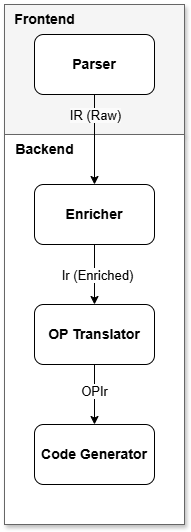
\includegraphics[height=0.3\textheight, keepaspectratio]{drawio/architettura_alto_livello.png}
  \caption{Architettura generale del compilatore di FusedStream.}
  \label{fig:compiler-architecture}
\end{figure}

Il \emph{frontend} ha il compito di analizzare l'espressione Scala della pipeline e di ricostruirne la struttura in una rappresentazione logica interna.
Il parser riconosce le sorgenti e gli operatori messi a disposizione dalla DSL e produce una prima rappresentazione della pipeline, denominata
\emph{Stream IR}. In questa fase la rappresentazione mantiene ancora una corrispondenza diretta con i concetti di alto livello del modello di streaming,
quali sorgenti, operazioni.

Il \emph{backend} riceve la rappresentazione prodotta dal frontend e la
trasforma progressivamente fino a ottenere il codice che implementa
concretamente la pipeline. La prima fase consiste nell'\emph{enrichment} della
Stream IR. Durante questa trasformazione vengono associate all'albero
informazioni necessarie alle fasi successive, tra cui variabili ausiliarie,
condizioni di terminazione e proprietà della pipeline. La struttura
risultante è un \emph{Enriched Stream IR}.

La Enriched Stream IR conserva ancora la semantica degli operatori di stream,
ma contiene informazioni sufficienti per determinare una strategia di
esecuzione. Essa viene quindi sottoposta a una seconda trasformazione,
che produce la \emph{Operation IR} (OP IR). Quest'ultima è costituita da operazioni più vicine
al codice imperativo da generare come dichiarazioni di variabili,
assegnamenti, condizioni, cicli, accessi ad array e operazioni necessarie
all'esecuzione parallela.

L'ultima fase è costituita dal \emph{code generator}, che effettua il lowering
della OP IR verso costrutti Scala concreti. A differenza di un compilatore
tradizionale, il risultato è un nuovo AST Scala. Tale AST viene restituito al
compilatore Scala e reinserito nel normale processo di compilazione del
programma.

Il flusso complessivo della trasformazione può quindi essere sintetizzato come:

\begin{equation*}
  \text{Scala AST}
  \longrightarrow
  \text{Stream IR}_{\mathrm{Raw}}
  \longrightarrow
  \text{Stream IR}_{\mathrm{Enriched}}
  \longrightarrow
  \text{OP IR}
  \longrightarrow
  \text{Generated Scala AST}.
\end{equation*}

\section{Architettura runtime}

\subsection{Il modello scelto}
Alla luce dei requisiti che non comprendono la necessità di effettuare zipping tra più stream e prediligono invece come obiettivo principe il massimo delle performance è stata naturale la scelta del modello \texttt{push}\ref{subsec:pushstream}

\subsubsection{Sintesi delle Operazioni supportate}

In Tabella~\ref{tab:stream_ops} viene riportato un quadro riassuntivo e delle caratteristiche delle operazioni analizzate.

\begin{table}[h!]
  \centering
  \caption{Confronto delle operazioni sui flussi di dati.}
  \label{tab:stream_ops}
  \vspace{2mm}
  \small
  \begin{tabular}{lcccc}
    \toprule
    \textbf{Operazione} & \textbf{Firma} & \textbf{Tipo di Trasformazione}     & \textbf{Cardinalità ($1:M$)} & \textbf{Gestione Stato} \\
    \midrule
    \textsf{Map}        & $A \to B$                 & $\mathcal{S}(A) \to \mathcal{S}(B)$ & $1 : 1$                      & Stateless               \\
    \textsf{Filter}     & $A \to \mathbb{B}$        & $\mathcal{S}(A) \to \mathcal{S}(A)$ & $1 : \{0,1\}$                & Stateless               \\
    \textsf{Limit}      & $\mathbb{N}_0$            & $\mathcal{S}(A) \to \mathcal{S}(A)$ & $1 : \{0,1\}$                & Stateful                \\
    \textsf{Skip}       & $\mathbb{N}_0$            & $\mathcal{S}(A) \to \mathcal{S}(A)$ & $1 : \{0,1\}$                & Stateful                \\
    \textsf{FlatMap}    & $A \to \mathcal{S}(B)$    & $\mathcal{S}(A) \to \mathcal{S}(B)$ & $1 : N$ ($N \ge 0$)          & Stateless  \\
    \bottomrule
  \end{tabular}
\end{table}

\subsection{Il runtime parallelo}

L'esecuzione parallela mantiene lo stesso modello \emph{push} adottato per l'esecuzione sequenziale. La parallelizzazione interviene sul modo in cui la sorgente viene attraversata: gli elementi vengono partizionati ed alaborati applicando la stessa pipeline fusa.
Data la funzione \(P\) che rappresenta una generica pipeline:

$$
P = o_n \circ o_{n-1} \circ \dots \circ o_1
$$

E una sorgente \(S\) partizionalible in maniera efficiente in \(k\) elementi:
$$
S = S_1 \cup S_2 \cup \dots \cup S_k,
$$

l'esecuzione sequenziale è banalmente:
$$
P(S),
$$

Nel caso parallelo, invece dato \(\oplus\) l'operatore che rappresenta la combinazione di risultati di una stream, possiamo rappresentare l'elaborazione come:

$$
P(S_1)\oplus\;P(S_2),\;\dots,\;\oplus P(S_k).
$$

A ciascuna partizione viene quindi applicato la stessa pipeline e i risultati intermedi vengono poi combinati. Alcuni combiner nativi nel caso parallelo non producono, strutture intermedie ma lavorano direttamente su memoria condivisa eliminando allocazioni intermedie
\subsubsection{Operazioni possibili con stream parallele}

La librerie rende possibile parallelizzare solamente con sorgenti e operatori per i quali il modello adottato consente di ottenere un'esecuzione prevedibilmente efficiente. Invece di permettere qualsiasi combinazione di sorgenti e operatori lasciando all'utente la responsabilità di valutarne l'effettiva convenienza, l'API impediscela costruzione di pipeline parallele considerate inadatte.

La restrizione costituisce quindi una scelta progettuale e non una semplice mancanza di funzionalità. L'obiettivo è guidare l'utente verso configurazioni per le quali il parallelismo rappresenti effettivamente una strategia di esecuzione appropriata.

\chapter{Design di dettaglio}

\section{Design dell'API pubblica}
\label{sec:api}

Particolare attenzione è stata posta nella progettazione dell'API pubblica della libreria.
L'obiettivo è stato quello di fornire un'interfaccia che garantisse contemporaneamente:

\begin{itemize}
  \item la possibilità di descrivere pipeline sufficientemente espressive
  \item l'estendibilità, in particolare per quanto riguarda le operazioni terminali
  \item il maggior numero possibile di garanzie a compile time
  \item la minimizzazione del codice necessario per verificare dinamicamente la correttezza
    delle combinazioni di operazioni richieste dall'utente.
\end{itemize}

Dal punto di vista concettuale, ogni stream può essere scomposto in tre componenti principali:

\begin{enumerate}
  \item una sorgente, generalmente costituita da una collezione o da un array;
  \item una sequenza di operazioni intermedie (\texttt{map}, \texttt{filter},\texttt{flatMap},..)
  \item un'operazione terminale
\end{enumerate}

La gerarchia di tipi esposta dall'API riflette direttamente questa struttura.
L'utilizzo di trait sealed, tipi parametrici, tipi opachi e vincoli sui parametri
di tipo permette di rappresentare a livello statico le proprietà della pipeline.
In questo modo il compilatore Scala può guidare l'utente durante la costruzione dello
stream e impedire le combinazioni non supportate.

Allo stesso tempo, l'API mantiene un certo grado di estendibilità, in particolare
consentendo all'utente di definire nuove operazioni terminali attraverso l'interfaccia
dei collector.

\subsection{Operazioni terminali}

Le operazioni terminali sono rappresentate attraverso l'astrazione \texttt{Collector}:

\begin{figure}[htbp]
  \centering

  \begin{tikzpicture}

    \umlclass[ type=selaed trait, alias=CollectorBase ]{CollectorBase$[$E, B, R$]$}
    {}
    {
      + supplier() : B \\
      + accumulator(buf : B, elem : E) : Boolean \\
      + finisher(buf : B) : R
    }

    \umlclass[ type=trait, alias=Collector, below=2cm of CollectorBase ]{Collector$[$E, B, R, S $<:$ TerminationPolicy$]$}
    {}
    {}

    \umlinherit{Collector}{CollectorBase}

  \end{tikzpicture}

  \caption{Gerarchia delle astrazioni \texttt{Collector} e \texttt{CollectorBase}.}
  \label{fig:collector-hierarchy}
\end{figure}

I quattro parametri di tipo rappresentano rispettivamente:

\begin{itemize}
  \item \texttt{E}: il tipo degli elementi ricevuti dallo stream;
  \item \texttt{B}: il tipo dello stato intermedio, o buffer, utilizzato durante l'accumulazione;
  \item \texttt{R}: il tipo del risultato finale prodotto dal collector;
  \item \texttt{S}: la politica di terminazione del collector.
\end{itemize}

Il metodo \texttt{supplier} crea lo stato iniziale utilizzato durante la raccolta,
mentre \texttt{accumulator} aggiunge un nuovo elemento, il valore booleano restituito
segnala che l'elaborazione può essere interrotta (si pensi a una findFirst).
Infine, \texttt{finisher} trasforma lo stato intermedio nel risultato finale.

La politica di terminazione è rappresentata mediante la seguente gerarchia:

\begin{figure}[htbp]
  \centering

  \begin{tikzpicture}

    \umlclass[type=sealed trait]{TerminationPolicy}{}{}

    \umlclass[type=sealed trait, below left=1.5cm and 1cm of TerminationPolicy]
    {Exhaustive}{}{}

    \umlclass[type=sealed trait, below right=1.5cm and 1cm of TerminationPolicy]
    {ShortCircuiting}{}{}

    \umlinherit{Exhaustive}{TerminationPolicy}
    \umlinherit{ShortCircuiting}{TerminationPolicy}

  \end{tikzpicture}

  \caption{Gerarchia delle politiche di terminazione.}
  \label{fig:termination-policy}
\end{figure}

Un collector \texttt{Exhaustive} richiede l'elaborazione dell'intero upstream,
mentre un collector \texttt{ShortCircuiting} può terminare non appena viene
soddisfatta una determinata condizione.

Ad esempio, i collector \texttt{toList} e \texttt{findFirst} hanno rispettivamente
i seguenti tipi:

\begin{lstlisting}[language=Scala]
toList[T]: Collector[T, ListBuffer[T], List[T], Exhaustive]
findFirst[T]: Collector[T, OptionBuffer[T], Option[T], ShortCircuiting]
\end{lstlisting}

Nel primo caso è necessario consumare tutti gli elementi dello stream prima di
produrre la lista risultante. Nel secondo caso, invece, il primo elemento ricevuto
è sufficiente a determinare il risultato e il collector può richiedere
l'interruzione anticipata della pipeline.
Questa proprietà viene codificata direttamente nel tipo del collector.

\subsubsection{Collector combinabili e parallelismo}

Per poter eseguire una riduzione in parallelo non è sufficiente che il collector
sia esaustivo. Gli stati intermedi prodotti indipendentemente dalle diverse
partizioni dello stream devono anche poter essere combinati, questa proprietà viene rappresentata dall'interfaccia:

\begin{lstlisting}[language=Scala]
trait Combinable[B] {
  def combine(left: B, right: B): B
}
\end{lstlisting}

Un collector utilizzabile come terminale di una pipeline parallela viene quindi definito come:

\begin{lstlisting}[language=Scala]
trait ParallelCollector[E, B, R]
    extends Collector[E, B, R, Exhaustive]
    with Combinable[B]
\end{lstlisting}

Il tipo \texttt{ParallelCollector} esprime pertanto staticamente due proprietà:

\begin{enumerate}
  \item la necessità di elaborare completamente lo stream;
  \item la possibilità di combinare i risultati intermedi ottenuti da più worker.
\end{enumerate}

Il type system permette così di distinguere un collector genericamente valido in
una pipeline sequenziale da un collector che possiede anche le proprietà
necessarie per essere utilizzato in una pipeline parallela.

\subsubsection{Collector specializzati}
Alcune operazioni terminali particolarmente comuni dispongono di un trattamento
specializzato da parte del compilatore di FusedStream. Due esempi sono
\texttt{toArray} e \texttt{summing}:

\begin{lstlisting}[language=Scala]
opaque type ToArrayCollector[T] <: ParallelCollector
opaque type SummingCollector[T <: Summable] <: ParallelCollector
\end{lstlisting}

I relativi metodi sono inoltre annotati con \texttt{@compileTimeOnly}:

Questi collector non vengono utilizzati come normali implementazioni runtime di
\texttt{Collector}. La loro presenza nella pipeline viene riconosciuta durante
l'espansione della macro e utilizzata per selezionare una strategia di code
generation dedicata.

Il tipo opaco permette di esporre verso l'esterno soltanto le proprietà rilevanti
del collector. Ad esempio, entrambi risultano essere sottotipi di
\texttt{ParallelCollector}, rendendoli compatibili con le pipeline parallele,
senza esporre all'utente i dettagli della strategia utilizzata internamente dal
compilatore.

La combinazione di tipi opachi e \texttt{@compileTimeOnly} permette quindi di
utilizzare il tipo del collector come protocollo di comunicazione tra l'API
pubblica e la macro di compilazione.

Nel caso di \texttt{toArray}, il compilatore può generare direttamente una
strategia di accumulazione specializzata evitando,
quando possibile, boxing e chiamate indirette attraverso l'interfaccia
\texttt{Collector}. Analogamente, \texttt{summing} può essere trasformato in una
riduzione diretta.

In questo modo l'API mantiene una sintassi uniforme:

\begin{lstlisting}[language=Scala]
stream.collect(Collector.toArray)
stream.collect(Collector.summing)
\end{lstlisting}

pur consentendo al compilatore di generare implementazioni sostanzialmente
differenti e specializzate per le singole operazioni terminali.

\subsection{Creazione dello stream: \texttt{from}}

La costruzione di una pipeline avviene a partire dal metodo \texttt{from}.
Oltre a identificare la sorgente degli elementi, il tipo restituito da
\texttt{from} determina quali modalità di esecuzione possono essere richieste
successivamente.

Non tutte le sorgenti possiedono infatti le caratteristiche necessarie per essere
sruttate parallelamente. L'API rappresenta questa proprietà attraverso il tipo restituito:
una sorgente per la quale è disponibile l'esecuzione parallela viene rappresentata
come un \texttt{ParallelizableSource[A]} (vedi \ref{fig:stream}).

Il metodo \texttt{parallel} non appartiene quindi genericamente a ogni
\texttt{Stream}, ma solamente alle sorgenti per le quali la libreria dichiara
esplicitamente il supporto alla parallelizzazione. Una pipeline costruita a partire da una sorgente non
parallelizzabile non può essere convertita in una \texttt{ParallelStream}, l'operazione semplicemente non è disponibile nel tipo
statico restituito all'utente.

\subsection{Tipologie di stream}

La modalità di esecuzione della pipeline è rappresentata attraverso una gerarchia
di tipi \texttt{sealed}:

\begin{lstlisting}[language=Scala]
sealed trait Stream[A]
sealed trait SequentialStream[A] extends Stream[A]
sealed trait ParallelizableSource[A] extends SequentialStream[A]
sealed trait ParallelStream[A]extends Stream[A]
\end{lstlisting}

\texttt{Stream[A]} rappresenta l'insieme minimo delle operazioni disponibili
indipendentemente dalla modalità di esecuzione:

\begin{lstlisting}[language=Scala]
def filter(p: A => Boolean): Stream[A]
def map[B](f: A => B): Stream[B]
def flatMap[B](f: A => SequentialStream[B]): Stream[B]
\end{lstlisting}

I sottotipi ridefiniscono (in maniera covariantemente) il tipo restituito dalle operazioni, ad esempio:

\begin{lstlisting}[language=Scala]
sealed trait ParallelStream[A] extends Stream[A] {
  override def filter(p: A => Boolean): ParallelStream[A]
  override def map[B](f: A => B): ParallelStream[B]
  override def flatMap[B](f: A => SequentialStream[B]): ParallelStream[B]
}
\end{lstlisting}

Una chiamata a \texttt{map} su una \texttt{ParallelStream[A]} produce quindi una
\texttt{ParallelStream[B]}, impedendo che l'informazione relativa alla modalità
di esecuzione venga persa lungo la pipeline.

Analogamente, una pipeline sequenziale:
\begin{lstlisting}[language=Scala]
sealed trait SequentialStream[A] extends Stream[A] {
  override def filter(p: A => Boolean): SequentialStream[A]
  override def map[B](f: A => B): SequentialStream[B]
  override def flatMap[B](f: A => SequentialStream[B]): SequentialStream[B]
  // Non supportati in stream paralleli
  def skip(n: Int): SequentialStream[A]
  def limit(n: Int): SequentialStream[A]
}
\end{lstlisting}

La posizione di \texttt{skip} e \texttt{limit} esclusivamente all'interno di
\texttt{SequentialStream} garantisce che queste operazioni non
risultuno disponibili su una \texttt{ParallelStream}.

\begin{figure}[htbp]
  \centering
  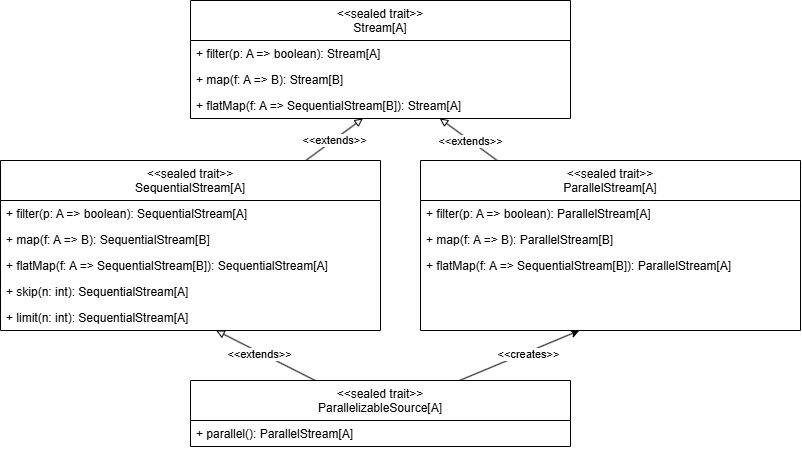
\includegraphics[width=0.8\textwidth]{drawio/stream.png}
  \caption{Diagramma UML delle classi per la gerarchia di Stream.}
  \label{fig:stream}
\end{figure}

\subsection{Operazione terminale \texttt{collect}}

L'operazione \texttt{collect} costituisce il punto nel quale la descrizione
della pipeline viene trasformata nel codice che ne realizza l'esecuzione.

La distinzione statica tra \texttt{SequentialStream} e \texttt{ParallelStream}
permette di imporre requisiti differenti sul collector terminale.

Una pipeline sequenziale può utilizzare genericamente un
\texttt{Collector}, mentre una pipeline parallela richiede un
\texttt{ParallelCollector}, cioè un collector esaustivo e dotato di una funzione
di combinazione dello stato intermedio. Le firme corrispondono quindi a:

\begin{lstlisting}[language=Scala]
// Sequential stream
collect(collector: Collector[E, B, R, S]): R

// Parallel stream
collect(collector: ParallelCollector[E, B, R]): R
\end{lstlisting}

Questa distinzione permette di rifiutare staticamente espressioni concettualmente
non valide come l'utilizzo di un collector short-circuiting non combinabile come
terminale di una pipeline parallela.

Ad esempio, un'operazione come:

\begin{lstlisting}[language=Scala]
stream
  .parallel()
  .collect(Collector.findFirst)
\end{lstlisting}

non soddisfa il vincolo richiesto da \texttt{ParallelCollector}, poiché
\texttt{findFirst} è tipato come:

\begin{lstlisting}[language=Scala]
Collector[
  T,
  OptionBuffer[T],
  Option[T],
  ShortCircuiting << non corretto
]
\end{lstlisting}

Al contrario:

\begin{lstlisting}[language=Scala]
stream
  .parallel()
  .collect(Collector.toArray)
\end{lstlisting}

è accettabile perché \texttt{ToArrayCollector[T]} è dichiarato come sottotipo
di \texttt{ParallelCollector}.
\begin{figure}[htbp]
  \centering
  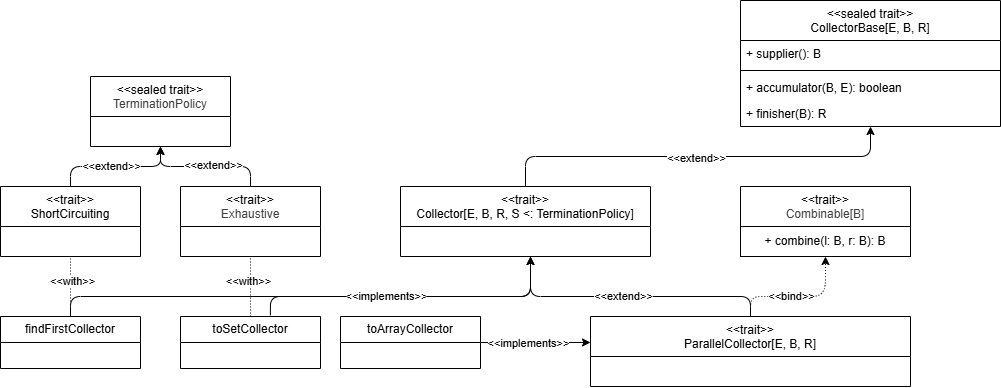
\includegraphics[width=0.8\textwidth]{drawio/collector.png}
  \caption{Diagramma UML delle classi per la gerarchia dei Collector e le relative TerminationPolicy.}
  \label{fig:collectors}
\end{figure}
\subsection{Configurazione compile-time e runtime}

La libreria distingue tra due tipologie di configurazione:
\texttt{CompileConfig}, relativa alle scelte che influenzano la generazione del
codice, e \texttt{RuntimeConfig}, relativa ai parametri utilizzati durante
l'esecuzione.

Entrambe le configurazioni sono gestite tramite il meccanismo dei \texttt{given}
di Scala. La libreria fornisce un comportamento di default, permettendo quindi
di utilizzare FusedStream senza alcuna configurazione esplicita nei casi più
comuni.

Quando necessario, l'utente può comunque sovrascrivere i valori predefiniti
fornendo una propria istanza \texttt{given} della configurazione desiderata nel
contesto della pipeline.

In questo modo l'API mantiene una configurazione implicita e poco invasiva,
lasciando comunque la possibilità di personalizzare sia il comportamento in fase
di compilazione sia quello in fase di esecuzione.

\subsection{Import semplificato dell'API}
Gli elementi dell'API pubblica vengono riesposti direttamente attraverso l'oggetto
\texttt{FusedStream}.
Questo permette di importare l'intera API necessaria con una singola istruzione:

\begin{lstlisting}[language=Scala]
import FusedStream.*
\end{lstlisting}

ottenendo così accesso sia alle funzioni per la costruzione delle pipeline sia ai
collector terminali pronti all'uso. L'obiettivo è mantenere l'interfaccia compatta e immediata, evitando che l'utente
debba conoscere o importare esplicitamente i diversi oggetti interni che compongono
l'API.

\section{Design della Stream IR}
\label{sec:stream-ir}

L'obiettivo della \emph{Stream Intermediate Representation} (Stream IR) è rappresentare la struttura logica di una pipeline e,permettere alle successive fasi del compilatore di associare all'albero nuove informazioni.

Il design della Stream IR è una struttura ad albero estensibile che prende ispirazione dal paper \emph{Trees That Grow}~\cite{najd2017trees}.

Il problema principale da gestire è che un Abstract Syntax Tree non rimane immutato durante l'intero processo di compilazione. Al contrario, le fasi del compilatore introducono informazioni da associare ai nodi dell'albero. Una possibile soluzione consiste nel definire una rappresentazione differente per ciascuna fase. Questo porterebbe però duplicazione di una parte considerevole della struttura dell'AST. Un altra opzione potrebbe essere avere un nodo unico per ogni fase con campi opzionali o un nodo base con varie estensioni per reappresentare le proprie fasi, questi approcci hanno però un problema: rendono più complicata e soggetta a possibili errori la gestione di questi dati.

E' stata invece creata una struttura parametrizzata a livello di tipo $P$ per determinare fase alla quale appartiene l'albero.

\begin{lstlisting}[language=Scala]
sealed trait Phase
object Phase {
  sealed trait Raw extends Phase
  sealed trait Enriched extends Phase
}
enum StreamTree[P <: Phase, A] {
  ...
}
\end{lstlisting}
\begin{description}
  \item[$A$] Rappresenta il tipo degli elementi prodotti dal nodo.
  \item[$P$] Identifica la fase del ciclo di vita (\texttt{Phase}) nella quale il nodo si trova.
\end{description}

L'utilizzo della fase come parametro di tipo, rende esplicito al type system quali rappresentazioni possono essere manipolate, ne derivano benefici come pattern matching esaustivo e garanzie a compile time.

Il passaggio tra il risultato del parser e dell'enricher quindi viene espresso direttamente attraverso i tipi.

\begin{center}
  \texttt{StreamTree[Phase.Raw, A]}
  \texttt{StreamTree[Phase.Enriched, A]}.
\end{center}

\subsection{Struttura dell'albero}
La Stream IR modella una pipeline come un albero i cui nodi corrispondono alle operazioni del dominio degli stream. Le sorgenti costituiscono la foglia
dell'albero.

Una rappresentazione semplificata della gerarchia è mostrata in
Figura~\ref{fig:stream-ir}.

\begin{figure}[htbp]
  \centering
  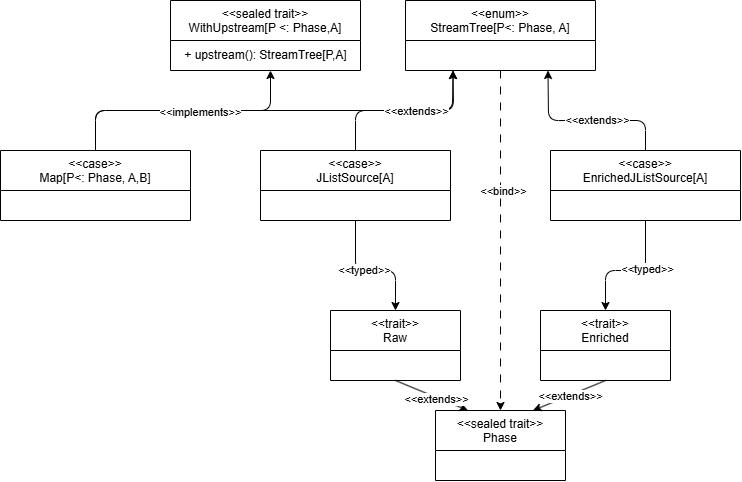
\includegraphics[height=0.3\textheight, keepaspectratio]{drawio/streamIr.png}
  \caption{Struttura semplificata della Stream IR.}
  \label{fig:stream-ir}
\end{figure}

Gli operatori che non modificano la propria rappresentazione tra le due fasi sono parametrizzati direttamente tramite $P$, Ad esempio \texttt{Map}:

\begin{lstlisting}[language=Scala]
case Map[P <: Phase, A, B](upstream: StreamTree[P, A],...) extends StreamTree[P, B]
\end{lstlisting}

Si noti come la fase del nodo impone anche la fase del relativo \emph{upstream} garantendo la correttezza dell'intera struttura dati

Gli operatori la cui struttura viene invece effettivamente estesa hanno varianti specifiche per fase. Un esempio dedicato al \texttt{flatMap} è riportato nella sezione a seguire.

\section{Rappresentazione per la Code Generation (OP Ir)}
\label{sec:op-ir}

La Stream IR descritta nella sezione precedente mantiene una rappresentazione di alto livello della pipeline e dei suoi operatori. Tale struttura è
particolarmente adatta alle analisi specifiche del dominio degli stream, ma non costituisce una rappresentazione conveniente per la generazione del codice.

Per questo si introduce una seconda rappresentazione intermedia, \emph{Operation IR} (OP IR). La traduzione verso questa rappresentazione costituisce un processo di \emph{lowering}: operatori di alto livello vengono eliminati e sostituiti da costrutti che descrivono esplicitamente il modello di esecuzione della pipeline. A differenza della Stream IR, la OP IR non modella quindi il dominio degli stream.

La rappresentazione è organizzata attorno a due categorie fondamentali: \emph{Values}, che descrivono espressioni che producono un valore, e \emph{Operations}, che descrivono azioni e strutture di controllo. Un programma nella OP IR è una sequenza di operazioni e un valore che ne costituisce il risultato:

\begin{lstlisting}[language=Scala]
case class Program[T](operations: List[Op], result: Value[T])
\end{lstlisting}

Questo ulteriore linguaggio intermedio permette di suddividere la generazione del codice in due fasi con responsabilità distinte. La prima opera sulla rappresentazione logica della pipeline e, sulla base degli operatori presenti, della sorgente, dell'operazione terminale e delle proprietà ricavate durante l'analisi, come la cardinalità e l'allineamento degli indici, determina la strategia di esecuzione più adatta e la esprime attraverso la OP IR.
La seconda fase è invece meccanica: opera su un insieme ristretto di primitive della OP IR e ne effettua il lowering nei corrispondenti costrutti Scala. Le decisioni relative a come implementare la pipeline sono quindi prese prima della generazione effettiva del codice.

\subsection{Valori}

I \emph{Values} rappresentano espressioni che producono un risultato e sono utilizzati come operandi dalle operazioni della OP IR.
La gerarchia è composta da innanzitutto valori elementari, come costanti o riferimenti a Simboli e da valori composti che descrivono operazioni su altri
valori come confronti, operazioni aritmetiche o applicazioni di funzioni, sono inoltre presenti valori specifici come accessi a array o iteratori.

Un \texttt{Value} descrive quindi un'espressione che può essere incorporata all'interno di una \texttt{Op}. Ad esempio, la condizione di un ciclo \texttt{While} è
rappresentata come un \texttt{Value[Boolean]}, mentre il valore assegnato da una \texttt{AssignVal} è a sua volta rappresentato tramite un \texttt{Value}. Un esempio parziale della gerarchie è presente in figura\ref{fig:values}

\begin{figure}[htbp]
  \centering
  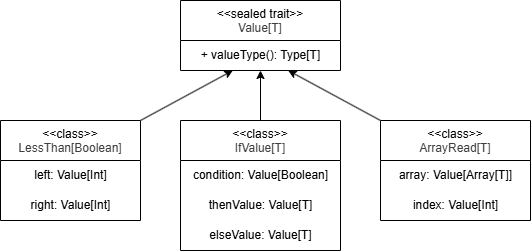
\includegraphics[height=0.3\textheight, keepaspectratio]{drawio/value.png}
  \caption{Struttura semplificata della Stream IR.}
  \label{fig:values}
\end{figure}

Ogni valore possiede l'informazione relativa al tipo che rappresentano, utilizzato durante la successiva generazione del codice.

\begin{lstlisting}[language=Scala]
sealed trait Value[T] {def valueType: Type[T]}

final case class LessThan(...) extends Value[Boolean] {
  override val valueType: Type[Boolean] = Type.of[Boolean]
}

final case class IfValue[T](
  ...
)(using val valueType: Type[T]) extends Value[T]

final case class ArrayType[T](
    ...
)(using val valueType: Type[Array[T]]) extends Value[Array[T]]
\end{lstlisting}

Il parametro di tipo permette di esprimere staticamente i vincoli, a livello di tipi tra le diverse primitive della IR. Per esempio in \texttt{LessThan}, entrambi gli operandi devono essere valori interi, mentre il risultato è necessariamente un \texttt{Value[Boolean]}.

La sola informazione contenuta nel parametro generico non è però sufficiente per la successiva generazione del codice, ogni \texttt{Value[T]} espone quindi anche un \texttt{Type[T]}, attraverso il campo \texttt{valueType}.

Si realizza così una forma di \emph{type capture}: oltre a conoscere staticamente che un nodo produce un valore di tipo \texttt{T}, la IR conserva
una rappresentazione del tipo utilizzabile dalle Scala Quotes. Per tipi noti in maniera statica, per valori parametrici viene invece propagata attraverso un parametro contestuale \texttt{Type[T]}.

TODO: sposta in lowering e linka
Questa informazione viene utilizzata durante il lowering per costruire
espressioni Scala correttamente tipizzate. Il code generator può infatti
recuperare il \texttt{Type} associato a un \texttt{Value} e renderlo
disponibile come \texttt{given Type[T]} durante la costruzione delle
\texttt{Expr[T]}. In questo modo la OP IR conserva le informazioni di tipo
necessarie alla generazione senza dover ricostruire il tipo a partire dalla
struttura del nodo.

\subsection{Operazioni}

Le \emph{Operations} rappresentano invece le azioni che costituiscono il corpo del programma generato.

La OP IR comprende operazioni elementari per la dichiarazione e l'aggiornamento dello stato, come \texttt{Declare}, \texttt{AssignVal} o
\texttt{Inc}. Il controllo del flusso è espresso esplicitamente attraverso \texttt{If} e \texttt{While}.

Sono inoltre presenti operazioni specializzate per le strategie di materializzazione utilizzate dalla libreria. \texttt{ArrayWrite}, ad esempio,
rappresenta direttamente la scrittura di un elemento in un array, mentre \texttt{DynamicArrayBuilderAdd} rappresenta l'inserimento in un buffer la cui
dimensione non è nota staticamente.

\section{La collection strategy}
\label{sec:collector_desion}

La fase terminale di una stream è rappresentata internamente attraverso una \texttt{CollectionStrategy}. Questa astrazione descrive la strategia con cui gli elementi prodotti dalla pipeline devono essere consumati e aggregati per ottenere il risultato finale.

\begin{figure}[htbp]
  \centering
  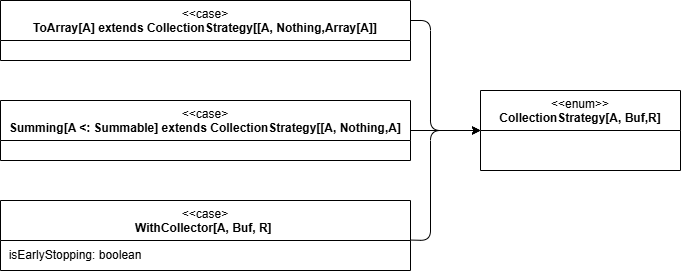
\includegraphics[width=0.8\textwidth]{drawio/collectionStrategy.png}
  \caption{Diagramma UML delle classi per la gerarchia \texttt{CollectionStrategy}.}
  \label{fig:coll_strat}
\end{figure}

L'introduzione di questa rappresentazione permette di separare il collector espresso dall'utente nella DSL dalla modalità con cui il compilatore genera il codice relativo all'operazione terminale. In particolare, i collector possono essere suddivisi in due categorie.

La prima comprende i \emph{collector concreti}, che forniscono direttamente l'implementazione delle operazioni necessarie alla raccolta. Tali operazioni vengono quindi invocate dal codice generato durante l'esecuzione della stream.

La seconda comprende invece i \emph{collector opachi}. Questi non costituiscono l'implementazione effettivamente utilizzata a runtime, ma agiscono come placeholder tipati all'interno della DSL. Il compilatore li riconosce durante il parsing e li sostituisce con una \texttt{CollectionStrategy} specializzata, la cui implementazione è definita direttamente all'interno della libreria. Appartengono a questa categoria, ad esempio, i collector utilizzati per le operazioni \texttt{toArray} e \texttt{summing}.

Questa distinzione consente quindi di specializzare le operazioni terminali note alla libreria, evitando di rappresentarle necessariamente attraverso il protocollo generale di un collector.

\chapter{Implementazione}

\section{Parsing}
La fase di parsing ha l'obiettivo di trasformare l'albero sintattico tipizzato prodotto dal compilatore Scala in una \texttt{StreamIR} (Sezione~\ref{sec:stream-ir}) e di estrarre, a partire dal collector (Figura~\ref{fig:collectors}), la corrispondente \texttt{CollectionStrategy}. Il parsing della pipeline e quello dell'operazione terminale sono mantenuti separati e vengono successivamente combinati nella rappresentazione utilizzata dalle fasi successive.

\subsection{Parsing della stream}
\label{sec:parsing}
Data una fused stream come:

\begin{lstlisting}[language=Scala]
  val result = FusedStream
    .from(numbers)
    .filter(i => i % 2 == 0)
    .skip(1)
    .map(i => i * 10)
    .collect(summing)
  \end{lstlisting}
\label{lst:filter_map}

l'obbiettivo della fase di parsing è ricondursi a una StreamIr del tipo:

\[
  \begin{aligned}
    \mathrm{ArraySource[Int]}
    & \xrightarrow{\;\mathrm{filter} : (Int \to Boolean)\;}
    \mathrm{Filter[Int]}
    \\
    & \xrightarrow{\;\mathrm{skip} : Int\;}
    \mathrm{Skip[Int]}
    \\
    & \xrightarrow{\;\mathrm{map} : (Int \to Int)\;}
    \mathrm{Map[Int,Int]}
  \end{aligned}
\]
(nota, non è presente il collector in quanto trattato a parte, vedi \ref{subsec:parsing_collector})

Il parsing è effettuato analizzando l'AST tipizzato esposto dalla reflection API, in particolare il codice in Listing\ref{lst:filter_map} produce:

\begin{lstlisting}[caption={Rappresentazione ad albero dell'AST di Scala}, label={lst:scala-ast}]
Inlined(
  None,
  Nil,
  Apply(
    TypeApply(
      Select(
        Apply(
          Select(
            Apply(
              Select(
                Apply(
                  TypeApply(
                    Select(Ident("FusedStream"), "from"),
                    List(Inferred())
                  ),
                  List(Ident("numbers"))
                ),
                "filter"
              ),
              List(
                Block(
                  List(
                    DefDef(
                      "$anonfun",
                      List(TermParamClause(List(ValDef("i", Inferred(), None)))),
                      Inferred(),
                      Some(
                        Apply(
                          Select(
                            Apply(
                              Select(Ident("i"), "%"),
                              List(Literal(IntConstant(2)))
                            ),
                            "=="
                          ),
                          List(Literal(IntConstant(0)))
                        )
                      )
                    )
                  ),
                  Closure(Ident("$anonfun"), None)
                )
              )
            ),
            "skip"
          ),
          List(Literal(IntConstant(1)))
        ),
        "map"
      ),
      List(Inferred())
    ),
    List(
      Block(
        List(
          DefDef(
            "$anonfun",
            List(TermParamClause(List(ValDef("i", Inferred(), None)))),
            Inferred(),
            Some(
              Apply(
                Select(Ident("i"), "*"),
                List(Literal(IntConstant(10)))
              )
            )
          )
        ),
        Closure(Ident("$anonfun"), None)
      )
    )
  )
)
\end{lstlisting}

\subsubsection{Rappresentazione dei nodi: ParsedTree}

\begin{figure}[htbp]
  \centering
  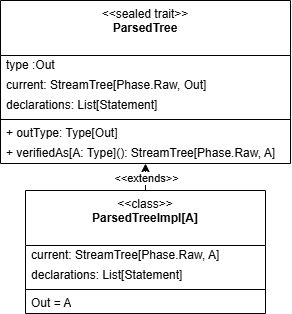
\includegraphics[height=0.3\textheight, keepaspectratio]{drawio/ParsedTree.png}
  \caption{Struttura per parsed tree}
  \label{fig:parsed_tree}
\end{figure}

Il trait \texttt{ParsedTree} rappresenta il risultato intermedio del parsing senza richiedere che il tipo di output sia noto al chiamante. Questo è necessario perché il tipo prodotto da una pipeline non è noto a priori, ma viene "scoperto" durante il parsing.

Per rappresentare questo tipo "nascosto", \texttt{ParsedTree} utilizza un abstract type member \texttt{Out}. Il tipo concreto viene fissato al momento della costruzione dell'implementazione, quando il tipo è noto. In questo modo il parser può esporre semplicemente un \texttt{ParsedTree}, mantenendo però internamente la correlazione tra il tipo dell'albero \texttt{current: StreamTree[Phase.Raw, Out]} e il relativo tipo di output.

Il tipo nascosto può essere utilizzato nelle successive fasi di parsing tramite un path-dependent type, ad esempio \texttt{type In = upstream.Out}. Il tipo precedentemente nascosto diventa così nuovamente utilizzabile per tipizzare operazioni successive, come una funzione \texttt{In => Boolean} per \texttt{filter} oppure \texttt{In => Out} per \texttt{map}.

Infine, \texttt{outType: Type[Out]} conserva l'evidenza reificata del tipo nascosto, necessaria per interagire con le API di \texttt{scala.quoted}, ad esempio per convertire un \texttt{Term} in una \texttt{Expr[In => Boolean]}.

\subsubsection{Il riconoscimento delle espressioni}

Il riconoscimento delle espressioni è effettuato tramite pattern matching

\begin{lstlisting}[caption={Pattern Matching sul Syntax Tree in Scala}]
private def parseTerm(expr: ir.quotes.reflect.Term): ParsedTree =
expr match
  // In caso di espressioni inlined analizza l'espressione sottostante
  case Inlined(_, _, inner) => parseTerm(inner)
  case Apply(TypeApply(NamedMethod("from"), _), List(arr)) => ...
  case Apply(TypeApply(NamedMethod("of"), _), List(arr)) => ...
  case Apply(Select(upstream, "filter"), List(predicate)) => ...
  case Apply(Select(upstream, "skip"), List(n)) => ...
  case Apply(Select(upstream, "limit"), List(n)) => ...
  case Apply(TypeApply(Select(upstream, "map"), List(outType)), List(mapper)) =>  ...
  case Apply(TypeApply(Select(upstream, "flatMap"), List(outType)), List(mapper)) => ...
  case Apply(Select(upstream, "parallel"), _) => parseTerm(upstream)
  // In caso di un blocco accumula le dichiarazioni e continua con il parsing
  case Block(blockStatements, expr) => parseTerm(expr) match {
    case ParsedTreeImpl(tree, decls) => ParsedTreeImpl(tree, blockStatements ++ decls)
  }
\end{lstlisting}

\subsubsection{Esempi di parsing specifico: filter}
Ogni caso poi tratta le informazioni ricevute ad esempio un filter è implementato come:
\begin{lstlisting}[caption={Parsing di un'operazione \texttt{filter}}]
  case Apply(...) => appendFilter(parseTerm(upstream, predicate))

  private def appendFilter(upstream: ParsedTree, predicateTerm: Term): ParsedTree = {
    type InOut = upstream.Out
    given Type[InOut] = upstream.outType
    val predicate = predicateTerm.asExprOf[InOut => Boolean]
    val filter = Filter[Phase.Raw, InOut](upstream.current, predicate, upstream.outType)
    ParsedTreeImpl[InOut](filter, upstream.declarations)
  }
\end{lstlisting}

Qui emerge un pattern ricorrente nel progetto: un tipo dipendente viene associato alla relativa evidenza reificata richiesta dalle API di \texttt{scala.quoted}.
Il tipo di output del nodo precedente viene definito localmente tramite \texttt{type InOut = upstream.Out}. Viene quindi resa disponibile un'istanza \texttt{Type[InOut]} a partire da \texttt{upstream.outType}. In questo modo il predicato e l'albero \texttt{upstream.current} condividono staticamente lo stesso tipo \texttt{InOut}, senza ricorrere a cast.
\subsubsection{Esempi di parsing specifico: flatMap}
Un caso più complesso è dato da \texttt{flatMap}. A differenza \texttt{filter} la funzione passata a \texttt{flatMap} produce a sua volta una \texttt{Stream}.
Tale stream deve quindi essere estratta dalla funzione e sottoposta ricorsivamente alla stessa procedura di parsing.

Si consideri, ad esempio:

\begin{lstlisting}[language=Scala]
FusedStream
  .from(numbers)
  .flatMap(x =>
    FusedStream.from(elements(x)).filter(y => y > 0)
  )
\end{lstlisting}

Il parametro \texttt{x} della funzione rappresenta l'elemento prodotto, a runtime, dall'upstream. Durante l'espansione della macro tale valore non è ancora disponibile; è tuttavia necessario per analizzare staticamente la stream interna.
A questo scopo viene creato una variabile di binding di tipo \texttt{In}, ovvero il tipo di output dell'upstream:

\begin{lstlisting}[language=Scala]
type In = upstream.Out
given Type[In] = upstream.outType
val flatMapBinder = createConstantIn
val elemRef = Ref(flatMapBinder).asExprOf[In]
\end{lstlisting}

Il simbolo non contiene quindi il valore effettivo dell'elemento, ma costituisce un placeholder tipizzato che lo rappresenta all'interno della IR.
La funzione ricevuta dal \texttt{flatMap} viene dapprima convertita nella corrispondente espressione tipizzata:

\begin{lstlisting}[language=Scala]
getType(outputType) match {
  case '[out] =>
  val function = functionTerm.asExprOf[In => Stream[out]]
  ...
}
\end{lstlisting}

Quello che si ottiene è una funzione del tipo:

$$
\mathrm{In} \rightarrow \mathrm{Stream[Out]}.
$$

A questo punto la funzione viene beta-ridotta contro il riferimento al binder:

\begin{lstlisting}[language=Scala]
val innerStreamExpr: Expr[Stream[out]] =
Expr.betaReduce {'{ $function($elemRef) }}
\end{lstlisting}

Ciò che si ottiene è quindi La stream interna che viene quindi sottoposta ricorsivamente a \texttt{parseTerm}. Si ottengono quindi due sottoalberi: l'upstream esterno e la stream interna prodotta dal \texttt{flatMap}. Il nodo della IR mantiene inoltre il simbolo del binder che collega i due:
Durante la successiva fase di code generation il binder verrà associato al valore dell'elemento corrente prodotto dall'upstream. In questo modo la stream interna può essere analizzata e ottimizzata durante la compilazione pur dipendendo da un valore che sarà disponibile soltanto a runtime.

\subsection{Parsing del collector}
\label{subsec:parsing_collector}
L'obiettivo di questa operazione è ricondursi a una collection strategy (vedi \ref{sec:collector_desion}) a partire dalla rappresentazione ricevuta. Il primo passo consiste nell'analizzarne il tipo associato all'espressione confrontadolo con i collector opachi  della libreria, se è questo il caso il parser costruisce direttamente la strategia specializzata corrispondente. Nel caso generale, invece, il collector fornito dall'utente deve essere preservato, viene quindi estratta la \emph{stop policy} per determinare staticamente se il collector supporti lo short-circuiting. Il risultato di questa analisi viene infine incorporato nella strategia generica \texttt{WithCollector}. La trasformazione può essere rappresentata come:

$$
\begin{aligned}
  \texttt{ToArrayCollector[A]}
  & \longrightarrow \texttt{ToArray[A]} \\[2mm]
  \texttt{SummingCollector[A]}
  & \longrightarrow \texttt{Summing[A]} \\[2mm]
  \texttt{CollectorBase[A, Buf, R]}
  & \longrightarrow
  \texttt{WithCollector[A, Buf, R]}
\end{aligned}
$$

Nota la tipizzazione su TerminationPolicy a questo punto viene persa, è infatti utilizzata solo per definire la grammatica della dsl e viene convertita nel valore booleano \texttt{isEarlyStopping} dentro \texttt{WithCollector}

\subsection{Parsing della configurazione statica}
La libreria effettua un'ulteriore operazione di parsing relativa alla configurazione di compilazione. A differenza del parsing della stream, basato sull'analisi del TASTy, in questo caso l'estrazione viene effettuata mediante quoted pattern matching. Poiché la configurazione deve essere interamente nota a compile time, i valori dei suoi campi devono poter essere estratti staticamente dall'espressione. Sono quindi accettate istanziazioni di \texttt{CompileConfig} i cui argomenti siano costanti note in fase di compilazione, come mostrato dal seguente \texttt{FromExpr}:

\begin{lstlisting}[caption={Unapplier con quoted pattern matching per configurazione statica}]
given FromExpr[CompileConfig] with {
  def unapply(expr: Expr[CompileConfig])(using Quotes): Option[CompileConfig] = {
    expr match {
      // CompileConfig(unsafe, logging)
      case '{ CompileConfig($u, $l) } =>
        for {
          unsafe <- u.value
          logging <- l.value
        } yield CompileConfig(unsafe, logging)

      // new CompileConfig(unsafe, logging)
      case '{ new CompileConfig($u, $l) } =>
        for {
          unsafe <- u.value
          logging <- l.value
        } yield CompileConfig(unsafe, logging)
    }
  }
}
\end{lstlisting}

\section{Enrichment}

\section{Traduzione in OPIr}

\section{Lowering}

\section{Traduzione end-to-end}

Quanto segue prova a ripercorrere passo passo il processo di analisi e generazione di codice della librerie, in particola a partire dalla stream (che utilizza una ArrayList come sorgente):

\begin{lstlisting}[language=Scala]
FusedStream.from(list)
  .map(f)
  .filter(p)
  .toArray
\end{lstlisting}

Una volta efettuato il parsing, la pipeline può essere rappresentata dalla seguente \texttt{StreamIr}:

$$
\operatorname{CollectionStrategy.ToArray}_{seq}
\left(
  \operatorname{Filter}_{p}
  \left(
    \operatorname{Map}_{f}
    \left(
      \operatorname{JListSource}(list)
    \right)
  \right)
\right).
$$

Durante l'enrichment diventa cc

La fase di planning, a partire dalla struttura definisce un piano di esecuzione del tipo:

$$
\boxed{
  \operatorname{While}
  \left[
    \boxed{
      y = f(x)
      \left[
        \boxed{
          \operatorname{IfValue}(p(y))
          \left[
            \boxed{
              \operatorname{ToArrayAppend}(y)
            }
          \right]
        }
      \right]
    }
  \right]
}
$$

Questa struttura viene quindi tradotta \texttt{OpIr}. La rappresentazione risultante è:

\begin{lstlisting}[
  language=OPIR,
  caption={OPIR generato per una pipeline con mapping, filtro e raccolta in array},
  label={lst:opir-example}
]
statements = [
  // Estrae la lista di origine
  Declare(source$macro$1,ScalaExpr(numbers)),
  // Estrae la size della lista
  Declare(sourceSize$macro$1,ScalaExpr(source$macro$1.size())),
  // Crea un vettore preallocato
  Declare(vec$macro$1,ArrayDefine[scala.Int](ScalaExpr(sourceSize$macro$1))),
  // Dichiara il counter e inizializza a 0
  Declare(i$macro$1,ConstantVal(0)),
  // Genera codice ottimizzato a runtime se e' una attaylist usiamo accesso indicizzato (costo o(1), niete iteratori)
  If(
    condition =IsInstanceOf[java.util.ArrayList[]](ScalaExpr(source$macro$1)),
    then =
      CodeBlock(
        Declare(i$macro$2,ConstantVal(0)),
        While(
          // Ciclo diretto su size, non abbiamo condizioni come limit o skip
          condition =LessThan(SymbolRef(i$macro$2),ScalaExpr(sourceSize$macro$1)),
          body =
            CodeBlock(
              // Leggiamo valore della list in una nuova variabile.
              // Se useUnsafe = true allora JListRead legge direttamente
              // l'array sottostante ad arraylist tramite varhandle
              Declare(elem$macro$1,
                      JListRead(ScalaExpr(source$macro$1),
                      SymbolRef(i$macro$2))),
              // Map
              CodeBlock(
                Declare(
                  mapped$macro$1,
                  ApplyFun(((i: scala.Int) => i.*(2)),SymbolRef(elem$macro$1))
                ),
                // Filter
                If(
                  condition =ApplyFun(
                        ((i: scala.Int) => i.%(2).==(0)),
                        SymbolRef(mapped$macro$1)),
                  then =
                    // Se la condizion e' risptettata write all'indice
                    CodeBlock(
                      ArrayWrite(
                        SymbolRef(vec$macro$1),
                        SymbolRef(i$macro$1),
                        SymbolRef(mapped$macro$1)),
                      Inc(i$macro$1)
                    )
                )
              ),
              Inc(i$macro$2)
            )
        )
      ),
    //codice non ottimizzato, per List senza accesso diretto, usa iteratore
    else =...
  )
],
result =  IfValue(
  // In base alla size dell'array lo ritorno direttamete o lo tronco
  Equal(SymbolRef(i$macro$1),ArrayLength(SymbolRef(vec$macro$1))),
  SymbolRef(vec$macro$1),
  ArrayTake(SymbolRef(vec$macro$1),SymbolRef(i$macro$1))
)
\end{lstlisting}

L'elenco di operazioni viene poi tradotto, durante il lowering nel bytecode java corrispondente (tramite CFR) a:

\begin{lstlisting}[language=java]
  ArrayList<Integer> numbers = new ArrayList<Integer>();
  numbers.addAll(List.of(..));

  int[] nArray;
  RuntimeConfig conff = RuntimeConfig$.MODULE$.default();
  ArrayList<Integer> source$macro$1 = numbers;
  int sourceSize$macro$1 = source$macro$1.size();
  int[] vec$macro$1 = new int[sourceSize$macro$1];
  int i$macro$1 = 0;
  if (source$macro$1 instanceof ArrayList) {
      ArrayList<Integer> list$proxy1 = source$macro$1;
      Object[] raw$macro$1 = ArrayListAccessor$.MODULE$.inline$ElementDataHandle().get(list$proxy1);
      for (int i$macro$2 = 0; i$macro$2 < sourceSize$macro$1; ++i$macro$2) {
          int elem$macro$1 = BoxesRunTime.unboxToInt(raw$macro$1[i$macro$2]);
          int mapped$macro$1 = elem$macro$1 * 2;
          if (mapped$macro$1 % 2 != 0) continue;
          vec$macro$1[i$macro$1] = mapped$macro$1;
          ++i$macro$1;
      }
  } else {
      // tramite foreach, rimosso per brevita'
  }
  if (i$macro$1 == vec$macro$1.length) {
      nArray = vec$macro$1;
  } else {
      Object object = Predef$.MODULE$.genericArrayOps(vec$macro$1);
      nArray = (int[])ArrayOps$.MODULE$.take$extension(object, i$macro$1);
  }
  int[] result = nArray;
\end{lstlisting}

\label{sec:lowring}

\chapter{Validazione e valutazione}
\section{Strategia di testing}
\subsection{Test funzionali}
\subsection{Test di compilazione}
\subsection{Copertura}

\section{Analisi del codice generato}
\subsection{Fusione delle operazioni}
\subsection{Inlining delle lambda}
\subsection{Boxing e allocazioni}
\subsection{Analisi del bytecode}

\section{Valutazione delle prestazioni}
\subsection{Metodologia}
\subsection{Baseline}
\subsection{Benchmark sequenziali}
\subsection{Benchmark paralleli}
\subsection{Allocazioni}

\chapter{Retrospettiva}

\bibliographystyle{plain}
\bibliography{references}
\end{document}
